\section{Methods}
\label{sec:methods}

To compute the coarse matrix $Ac$, a triple matrix multiplication should be done:
\begin{equation}
 Ac = R \times A \times P
\end{equation}
in which $R = P^T$. We do it in two parts, performing matrix-matrix multiplications (\matmult) twice: first $A \times P$, then $R \times B$, in which $B = A \times P$.

The matrices are partitioned on multiple processors by row blocks (Figure~\ref{fig:partition}). Matrices $A$ and $P$ have the same number of rows and consequently are partitioned the same way. $R$ has less number of rows and has a different partition.

\begin{figure}[tbh]
 \centering
 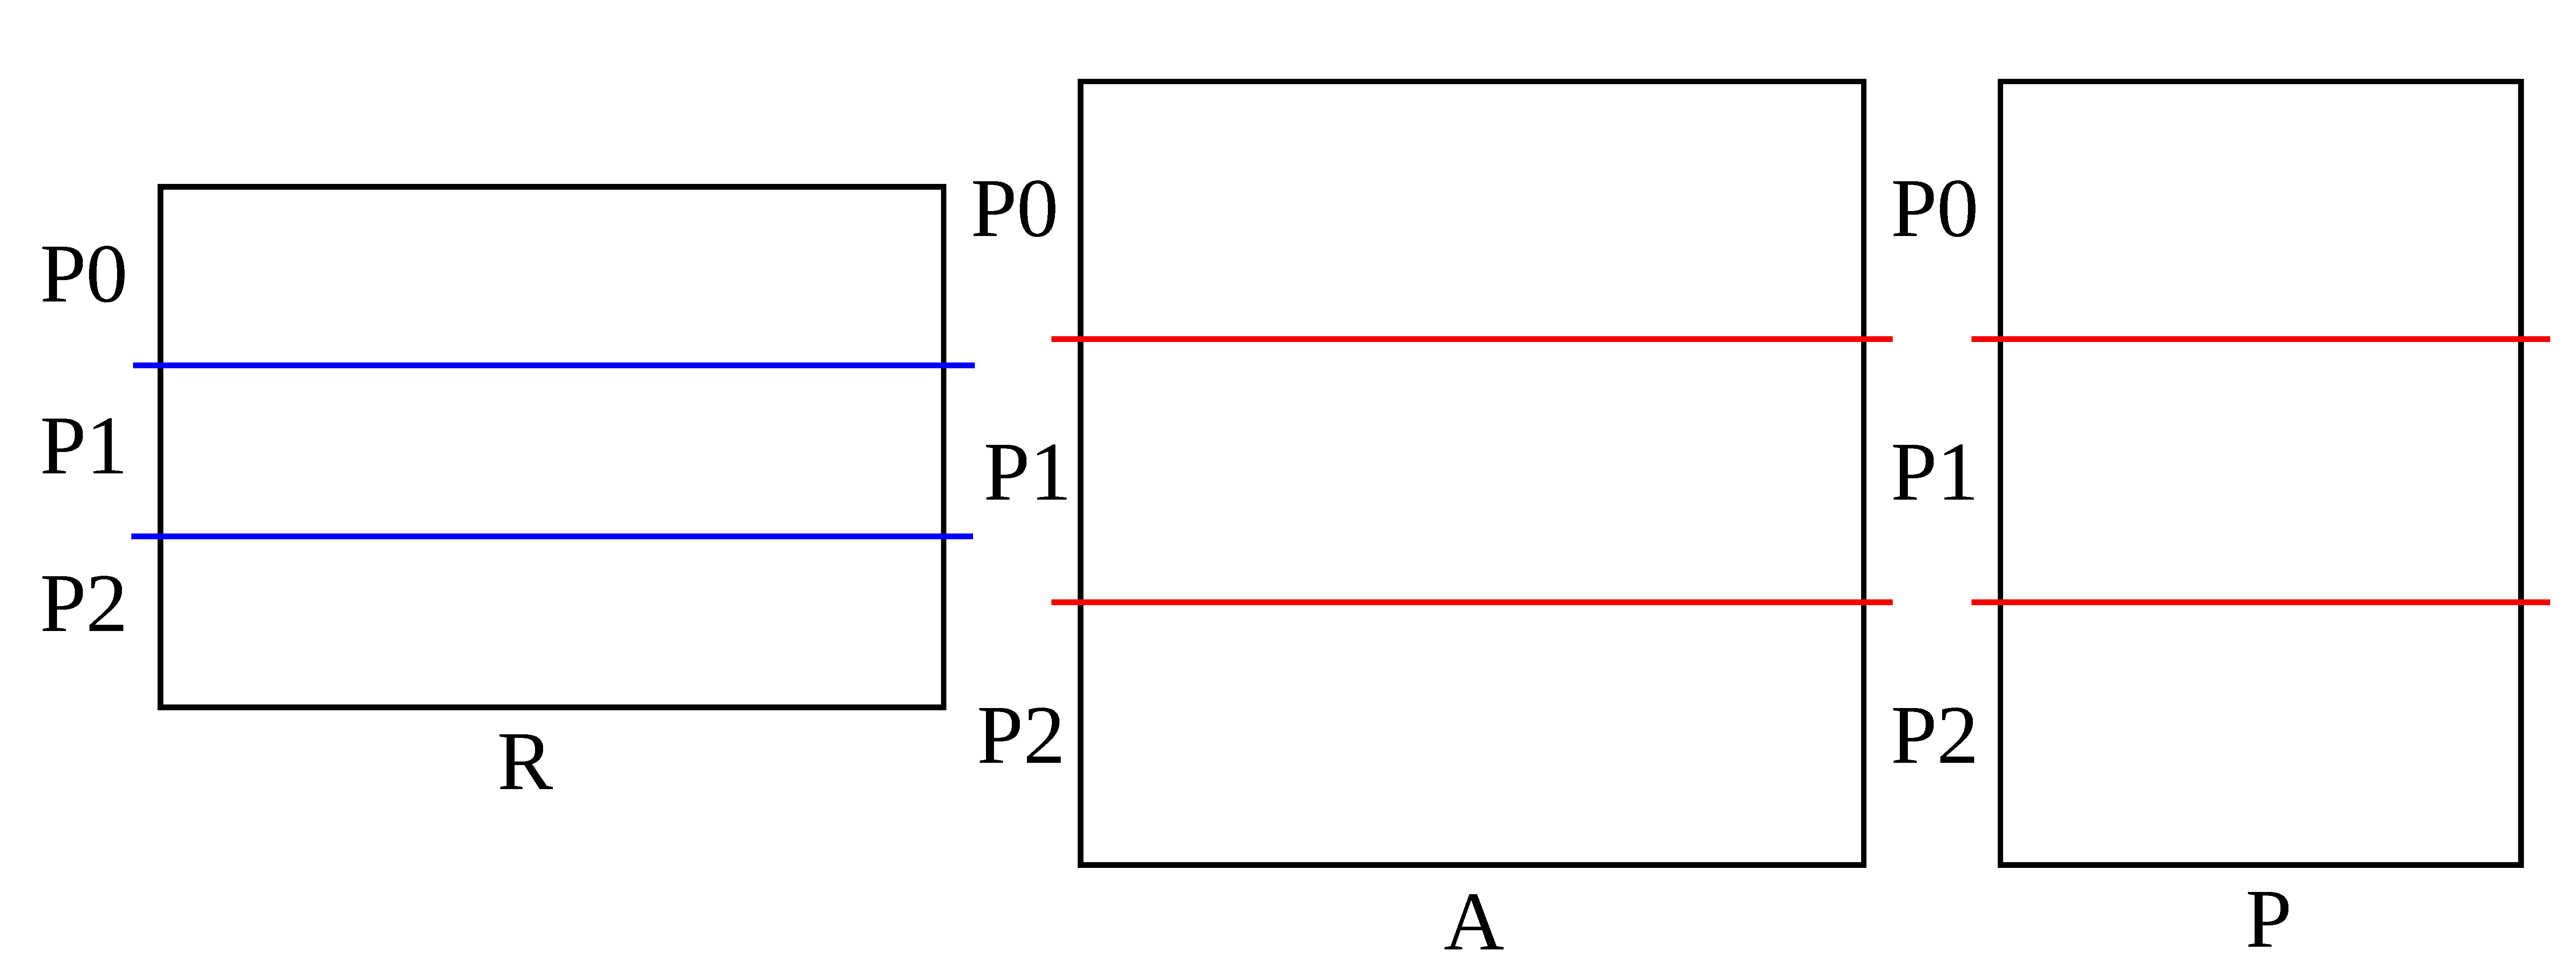
\includegraphics[width=8cm,height=3cm]{./figures/partition.pdf}
 \caption{}
 \label{fig:partition}
\end{figure}

\subsection{Part 1}

In this part we compute $B := A \times P$. We assume the same partition of rows of $A$ on its columns. The same partition of rows of $R$ is assumed on columns of $P$ (Figure~\ref{fig:part1}).

\begin{figure}[tbh]
 \centering
 \includegraphics[width=5.5cm,height=3cm]{./figures/part1.pdf}
 \caption{}
 \label{fig:part1}
\end{figure}

Here we consider doing \matmult on processor $P1$. To compute $B(i, j)$, we need to multiply row $i$ of $A$ with column $j$ of $P$ and add them together (we only consider the nonzeros).

\begin{figure}[tbh]
 \centering
 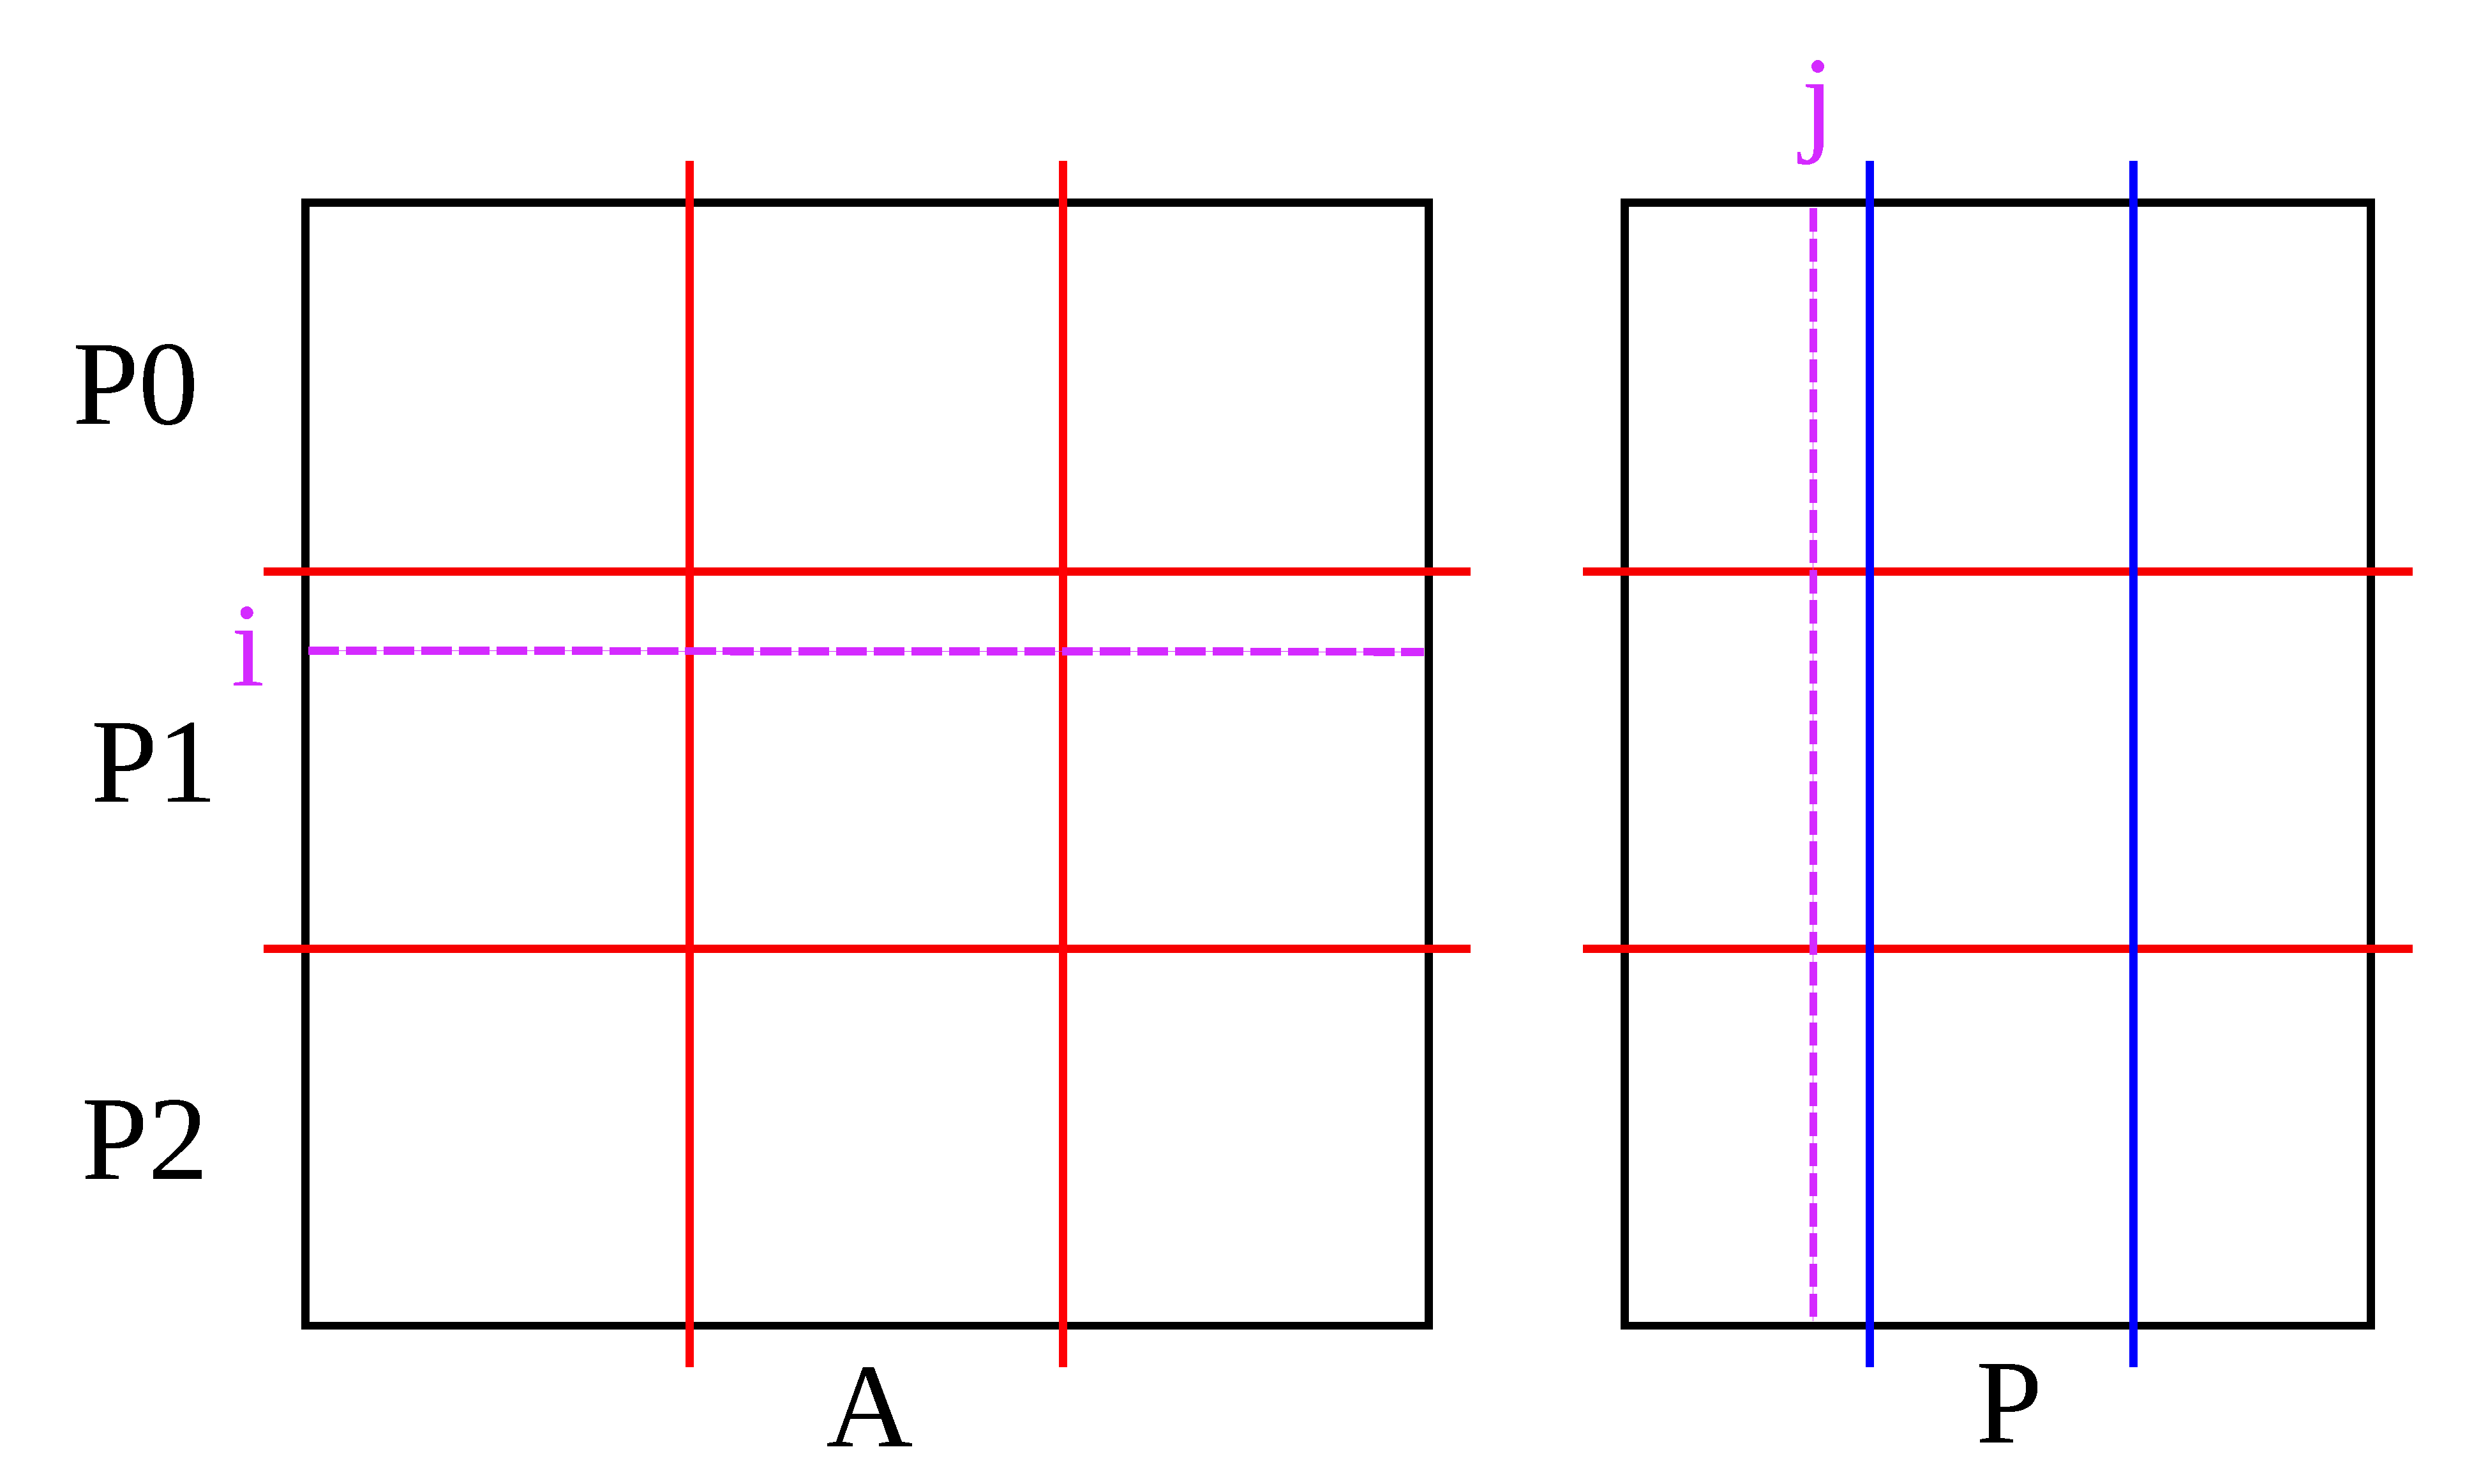
\includegraphics[width=5.5cm,height=3cm]{./figures/part1b.pdf}
 \caption{}
 \label{fig:part1b}
\end{figure}

Column $j$ is distributed between processors, so we will be able to perform the last summation at the end. (explain this part more and show why this method is not good). To avoid this, we can use the fact that $R$ is the transpose of $P$ and we already have computed it. We note that column blocks of $P$ (e.g. $r0$ in Figure~\ref{fig:part1c}) are actually row blocks of $R$ transposed ($rt0$, which is transpose of $r0$).

\begin{figure}[tbh]
 \centering
 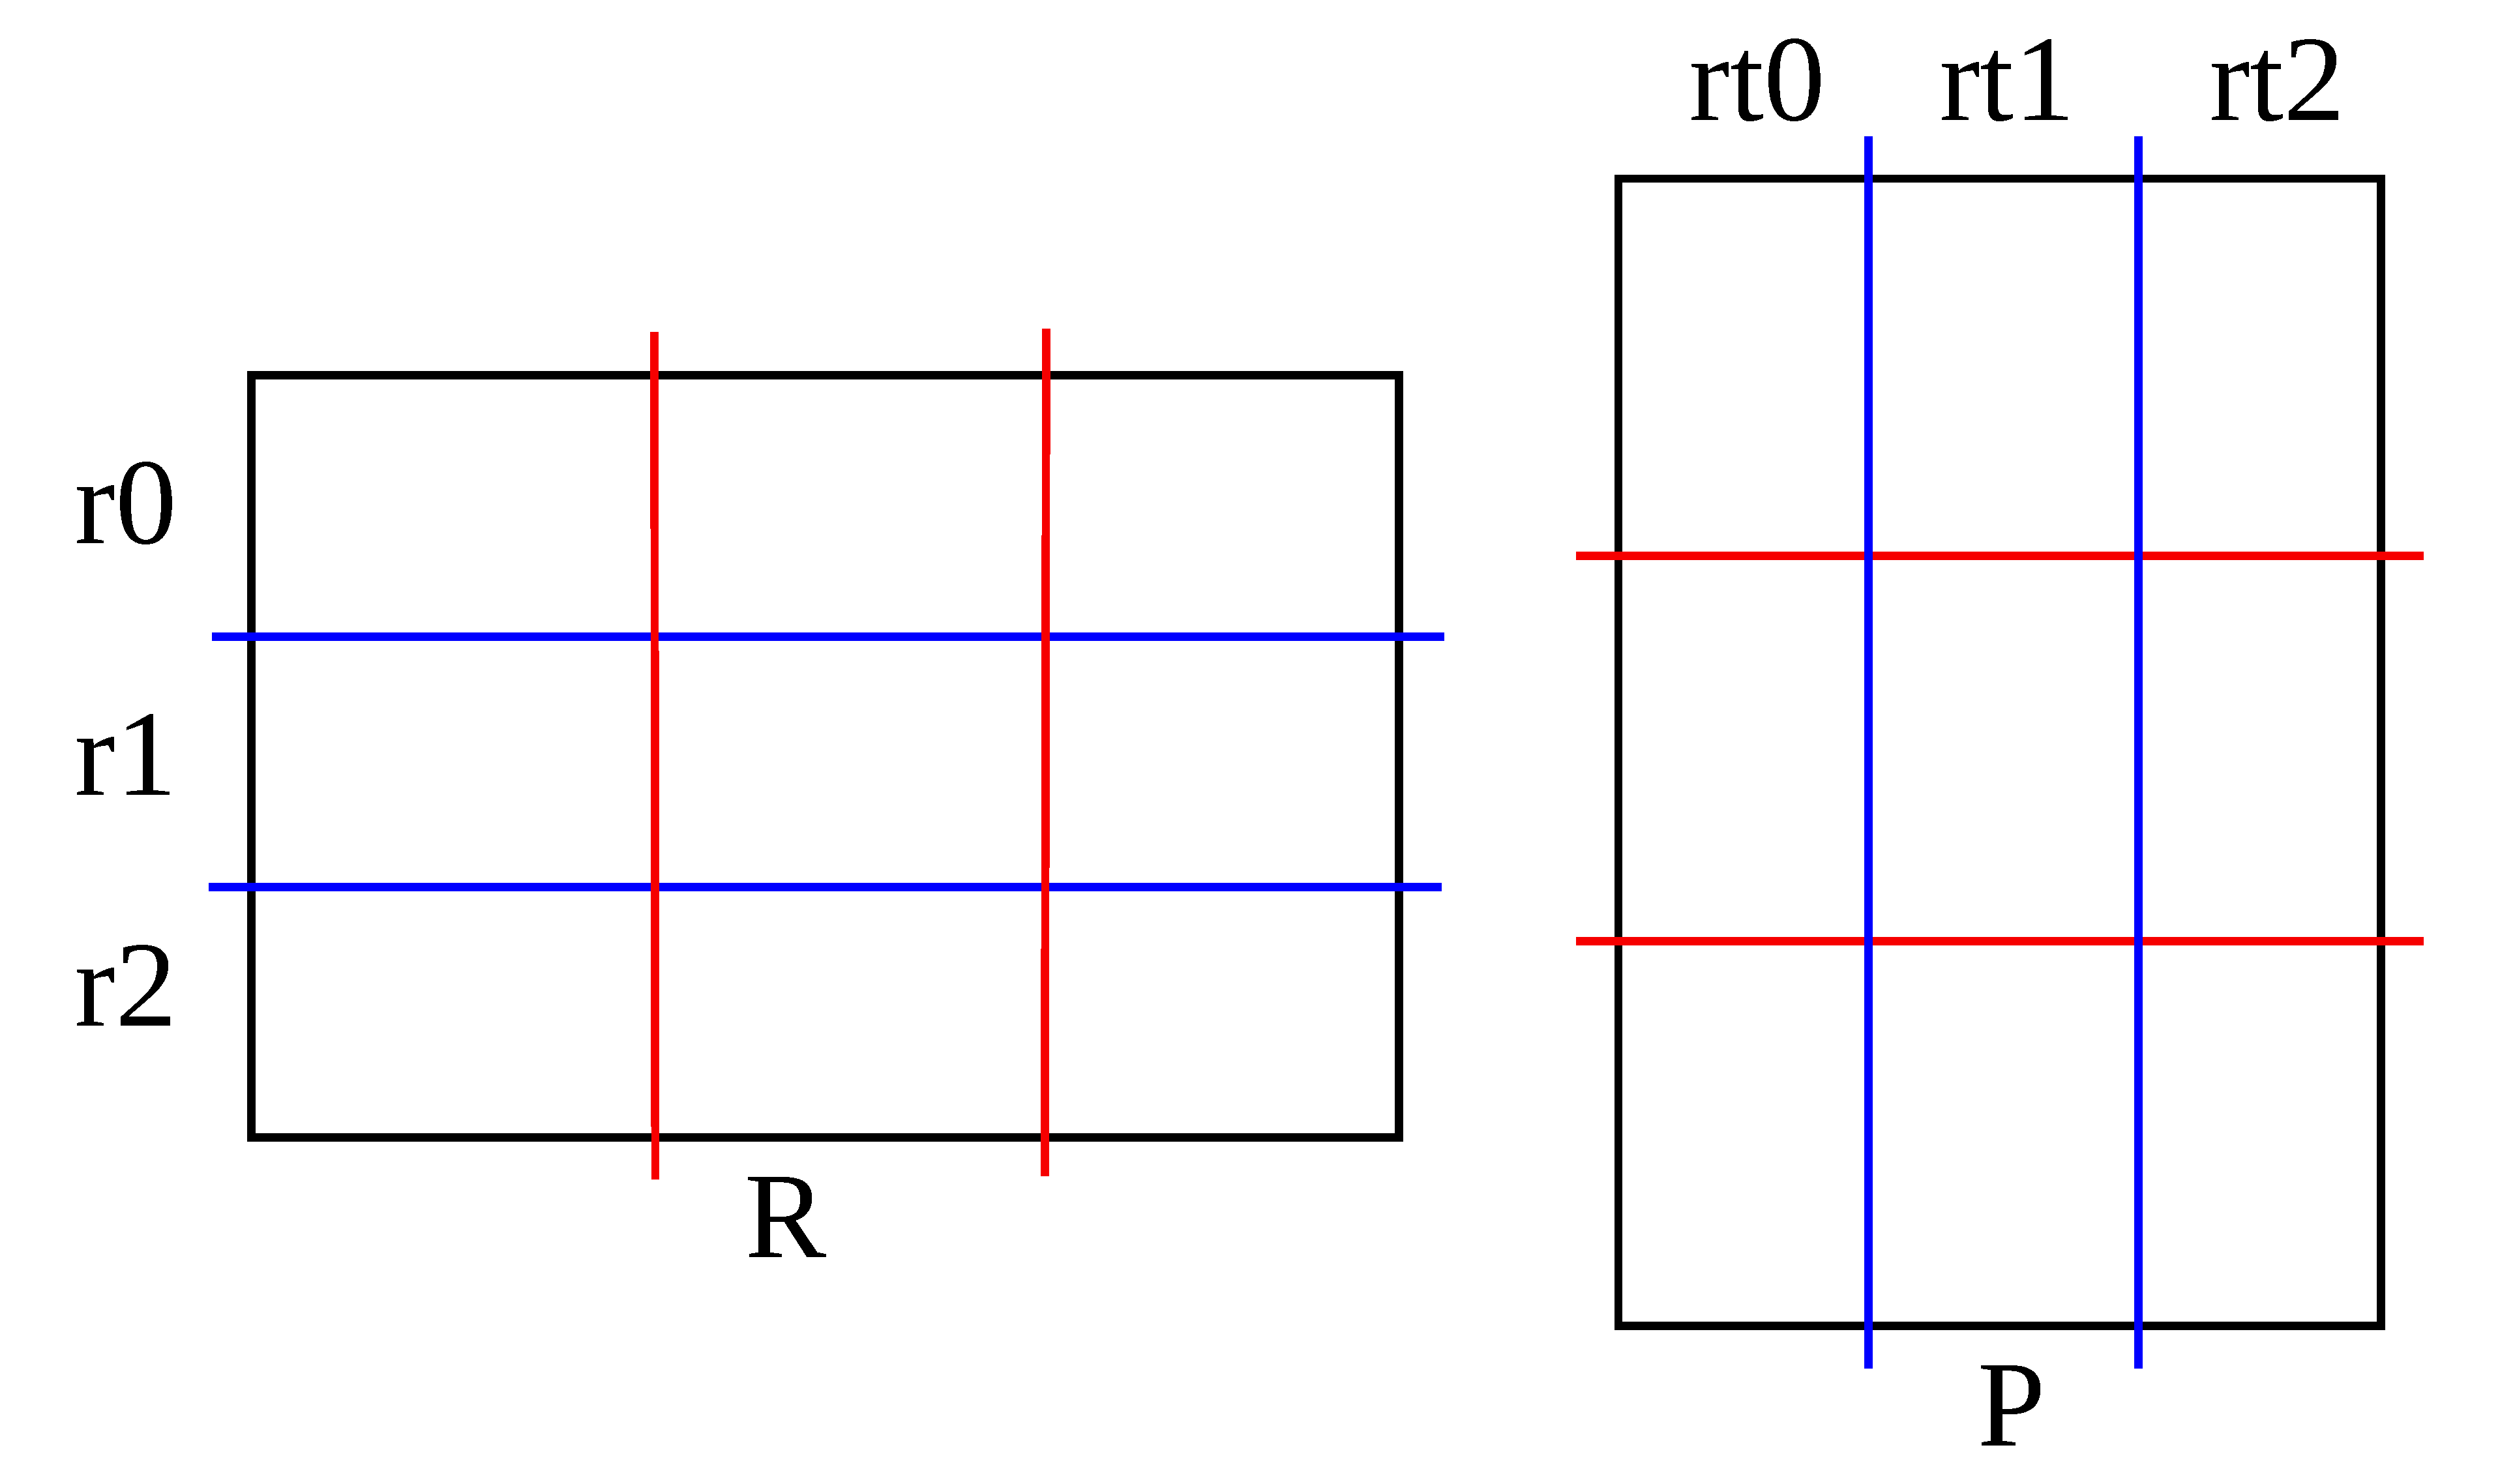
\includegraphics[width=5.5cm,height=3cm]{./figures/part1c.pdf}
 \caption{}
 \label{fig:part1c}
\end{figure}

$A_i$ is row block of $A$ on processor $i$.

\begin{algorithm}[H] 
  %\footnotesize
  \caption{Part 1: $B_i = A_i \times P$} \label{alg:part1} 
  \begin{algorithmic}[1]
    \Require $A_i$, $R$
    \Ensure  $B_i$ (result of $A_i \times P$)
    \State $RT_i \leftarrow$ compute transpose of $R_i$ (locally)
    \State $R2 \leftarrow RT_i$
    \For{$k=myrank:myrank+nprocs$}
      \State $R1 \leftarrow\ Irecv\ RT\ from\ right\ neighbor$
      \State $Isend(R2)\ to\ left\ neighbor$
      \State $B_j \leftarrow A_i \times R2$
      \State $wait\ for\ Isend\ and\ Irecv\ to\ finish$
      \State $swap(R1,R2)$
    \EndFor
  \end{algorithmic}
\end{algorithm}



\subsection{Part 2}
